\section{Sockets and Data Path}

\begin{frame}[fragile]{Sockets}
	\begin{columns}
		\column{0.15\textwidth}
			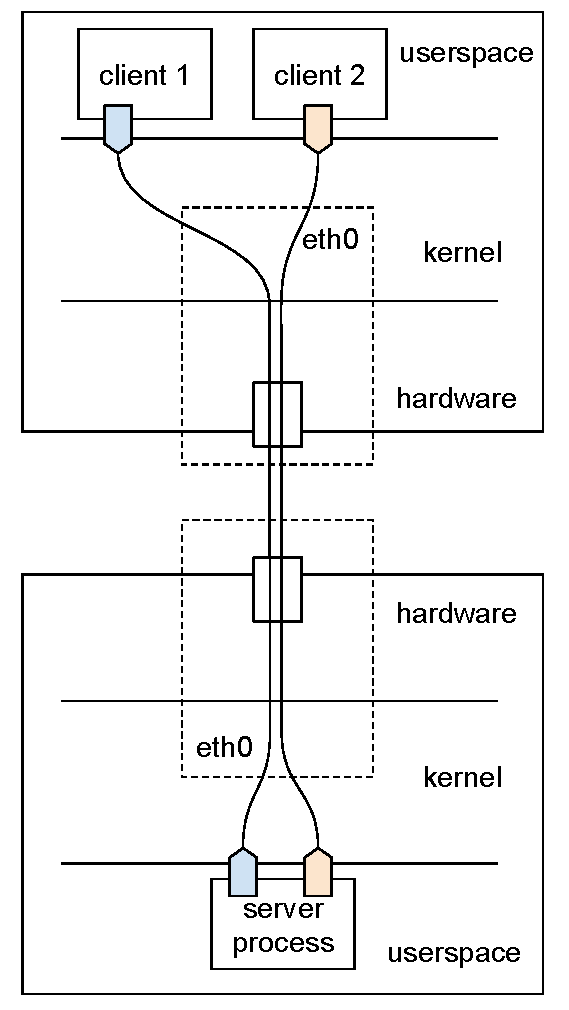
\includegraphics[width=1.4\textwidth]{slides/networking-socket/socket.pdf}
		\column{0.85\textwidth}
		\begin{itemize}
		\item The Socket programming model stems from \textbf{UNIX}
		\item It has been the main way for users to transmit data through the network since then
		\item Sockets are about more than networking, their behaviour depends on their attributes.
		\item A socket is represented from userspace as a \textbf{file descriptor} : \\
			\begin{minted}{c}
int socket(int domain, int type, int protocol);
			\end{minted}
				\begin{itemize}
					\item see \manpage{socket}{2}
				\end{itemize}
		\item The \code{domain} or \textit{family} defines the \textbf{underlying protocol} : IPv4, IPv6, Bluetooth, Netlink...
		\item The \code{type} defines the \textbf{semantics} : Connection-oriented, re-transmission, message ordering...
		\item The \code{protocol} depends on the domain and type, for further configuration.
		\end{itemize}
	\end{columns}
\end{frame}

\begin{frame}{Socket Families}
	\center{\code{int socket(}{\color{orange}int domain}\code{, int type, int protocol);}}
	\vspace{1cm}
	\begin{itemize}
		\item Familes as defined by \textbf{UNIX}, \textbf{POSIX} or are \textbf{Linux}-specific
		\item In Linux, defined in \code{include/linux/socket.h}
			\begin{itemize}
				\item \code{AF_UNIX}, \code{AF_LOCAL} : Unix Domain Sockets, for IPC. See \manpage{unix}{7}
				\item \code{AF_INET}, \code{AF_INET6} : IPv4 and IPv6 sockets, see \manpage{ip}{7}
				\item \code{AF_PACKET} (\textit{raw} sockets) : Layer 2 sockets, see \manpage{packet}{7}
				\item \code{AF_NETLINK}, \code{AF_ROUTE} : Userspace to kernel sockets for configuration, see \manpage{netlink}{7}
				\item More specialised families : \code{AF_BLUETOOTH}, \code{AF_IEE802154}, \code{AF_NFC}, etc.
			\end{itemize}
		\item Socket families are named \code{AF_xxx}, but equivalent names \code{PF_xxx} also exist
			\begin{itemize}
				\item \code{PF} standing for \textbf{P}rotocol \textbf{F}amily, \code{AF} for \textbf{A}ddress \textbf{F}amily
				\item legacy from the early UNIX days, \code{AF} and \code{PF} enums are equivalent on linux.
			\end{itemize}
	\end{itemize}
\end{frame}

\begin{frame}{Socket Types}
	\center{\code{int socket(int domain, }{\color{orange}int type}\code{, int protocol);}}
	\begin{itemize}
		\item Socket types indicates the transmission semantics, which usually means Layer 4
		\item Its meaning depends on the selected \textbf{domain} :
			\begin{itemize}
				\item \code{socket(AF_INET, SOCK_DGRAM, 0)} : UDP over IPv4 socket
				\item \code{socket(AF_UNIX, SOCK_DGRAM, 0)} : Message-oriented Unix Socket
			\end{itemize}
		\item \code{SOCK_STREAM} : Sequenced, reliable, two-way, connection-oriented
			\begin{itemize}
				\item \code{socket(AF_INET, SOCK_STREAM, 0)} : TCP over IPv4 socket
			\end{itemize}
		\item \code{SOCK_DGRAM} : Transmit datagrams of fixed maximum size, unreliable, connection-less
			\begin{itemize}
				\item \code{socket(AF_INET, SOCK_DGRAM, 0)} : UDP over IPv4 socket
			\end{itemize}
		\item \code{SOCK_RAW} : Raw sockets, usually containing the full \textbf{frame} including L2
		\item \code{SOCK_SEQPACKET}, \code{SOCK_RDM} : Other types with different ordering and message-length attributes
		\item \code{SOCK_NONBLOCK}, \code{SOCK_CLOEXEC} : Extra bitwise flags for configuration

	\end{itemize}
\end{frame}

\begin{frame}{Socket protocol}
	\center{\code{int socket(int domain, int type, }{\color{orange}int protocol}\code{);}}
	\vspace{1cm}
	\begin{itemize}
		\item Complements the tuple \code{<domain, type>} to allow protocol selection.
			\begin{itemize}
				\item \code{socket(AF_INET, SOCK_STREAM, 0)} : TCP over IPv4 socket
				\item \code{socket(AF_INET, SOCK_STREAM, IPPROTO_SCTP)} : SCTP over IPv4 socket
			\end{itemize}
		\item For \textbf{raw sockets}, allows filtering by Ethertype (in network byte order)
			\begin{itemize}
				\item \code{socket(AF_PACKET, SOCK_RAW, htons(ETH_P_ALL))} : All raw frames
				\item \code{socket(AF_PACKET, SOCK_RAW, htons(ETH_P_IP))} : All IPv4 frames
				\item \code{socket(AF_PACKET, SOCK_RAW, htons(ETH_P_8021Q))} : All Vlan frames
			\end{itemize}


	\end{itemize}
\end{frame}

\begin{frame}[fragile]{binding a socket}
	\center{\code{int bind(int sockfd, const struct sockaddr *addr, socklen_t addrlen);}}
	\begin{itemize}
		\item The \code{bind()} call allows associating a \textbf{local address} to a socket, see \manpage{bind}{2}
		\item For connection-oriented, necessary before being able to \textbf{accept} connections
		\item The socket's address format is represented by the generic \code{struct sockaddr}.
	\end{itemize}
		\begin{minted}{c}
struct sockaddr {
        sa_family_t sa_family;
        char        sa_data[14];
}
		\end{minted}
	\begin{itemize}
		\item The sockaddr must be subclassed by \textbf{family-specific} addresses :
	\end{itemize}

		\begin{minted}{c}
struct sockaddr_in {
        sa_family_t    sin_family; /* address family: AF_INET */
        in_port_t      sin_port;   /* TCP/UDP port in network byte order */
        struct in_addr sin_addr;   /* IPv4 address (uint32_t) */
};
		\end{minted}

\end{frame}

\begin{frame}{listen(), connect() and accept()}

\code{int listen(int sockfd, int backlog)}
	\begin{itemize}
		\item Set the socket as listening for up to \code{backlog} connections, \manpage{listen}{2}
	\end{itemize}
	\vspace{0.5cm}
\code{int accept(int sockfd, struct sockaddr *addr, socklen_t *addrlen)}
	\begin{itemize}
		\item Accepts a remote connection request on a \textbf{listening} socket, \manpage{accept}{2}
		\item The peer's address is filled into the \code{addr} parameter
		\item Returns a \textbf{new socket file descriptor} for that connection
	\end{itemize}
	\vspace{0.5cm}
\code{int connect(int sockfd, const struct sockaddr *addr, socklen_t addrlen)}
	\begin{itemize}
		\item Connect to a remote listening socket, \manpage{connect}{2}
		\item For connection-less protcols, it simply sets the destination address for datagrams
	\end{itemize}
\end{frame}

\begin{frame}{socket options}
	\begin{itemize}
		\item The \code{socket()} syscall doesn't allow fine-tuned configuration
		\item Sockets are configured through \code{setsockopt}
			\begin{itemize}
				\item \code{int setsockopt(int sockfd, int level, int optname, const void *optval, socklen_t optlen)}
				\item \manpage{setsockopt}{2}
			\end{itemize}
		\item The options can be used to configure the socket itself :
			\begin{itemize}
				\item \code{setsockopt(fd, SOL_SOCKET, ...);}
				\item \code{SO_ATTACH_BPF} : attach BPF programs to sockets
				\item \code{SO_BINDTODEVICE} : bind the socket to an interface
				\item see \manpage{socket}{7}
			\end{itemize}
		\item We can also configure the underlying protocol's behaviour :
			\begin{itemize}
				\item \code{setsockopt(fd, proto_num, ...);}
				\item The protocol number can be retrieved from \code{/etc/protocols}
				\item See \manpage{ip}{7}, \manpage{tcp}{7}, \manpage{udp}{7}, etc.
			\end{itemize}
	\end{itemize}
\end{frame}

\begin{frame}{Socket queues}
	\begin{itemize}
		\item All sockets are created with 2 queues : A \textbf{Receive} queue and a \textbf{Transmit} queue
		\item Queues size is the same for every socket at creation time, but can be adjusted
			\begin{itemize}
				\item With the \code{SO_RCVBUF} socket option, see \manpage{socket}{7}
				\item Using the \code{net.core.rmem_default} sysctl
			\end{itemize}
		\item Packets that can't be queued because the queue is full are dropped
		\item \code{netstat} shows the current queue usage of every open socket
	\end{itemize}
\end{frame}

\begin{frame}{read() and write()}
\begin{itemize}
	\item Generic syscalls, acting on any kind of file descriptors
	\item Does not allow passing any extra flags
\end{itemize}
\code{ssize_t read(int fd, void *buf, size_t count)}
	\begin{itemize}
		\item Reads up to \code{count} bytes from the socket.
		\item May block until data arrives, unless the socket is non-blocking
	\end{itemize}
	\vspace{0.5cm}
\code{ssize_t write(int fd, const void *buf, size_t count)}
	\begin{itemize}
		\item Only works on \textbf{connected} sockets
		\item Recipient's address is part of the socket's connection information
		\item For \textbf{datagrams}, \code{count} can't exceed the datagram size
		\item Not possible to know if the recipient actually received the message
	\end{itemize}
\end{frame}

\begin{frame}{send() and recv()}
\begin{itemize}
	\item Socket-only, very similar to read() and write()
	\item Also only works with \textbf{connected} sockets
	\item Accepts \code{MSG_xxx} bitwise flags
\end{itemize}
\code{ssize_t recv(int sockfd, void *buf, size_t len, int flags)}
	\begin{itemize}
		\item Similar to \code{read()}
		\item \code{MSG_PEEK} : Receives a message without consuming it from the socket queue
		\item \code{MSG_TRUNC} : Returns the real size, even if \code{count} is too small
		\item \code{MSG_DONTWAIT} : Per-message non-blocking operation
	\end{itemize}
	\vspace{0.5cm}
\code{ssize_t send(int sockfd, const void *buf, size_t len, int flags)}
	\begin{itemize}
		\item Accepts a remote connection request on a \textbf{listening} socket
		\item \code{MSG_MORE} : More data is yet to be sent, as a single datagram or TCP message
	\end{itemize}

\end{frame}

\begin{frame}{sendto() and recvfrom()}
	\begin{itemize}
		\item Socket-only, specifies the peer address per-message
		\item Allows using the same socket with multiple peers on UDP
	\end{itemize}
\code{ssize_t recvfrom(int sockfd, void *buf, size_t len, int flags,}
\code{                 struct sockaddr *src_addr, socklen_t *addrlen)}
	\begin{itemize}
		\item Get the address of the peer that sent the message along with the message
		\item \code{src_addr} and \code{addrlen} may be null, equivalent to \code{recv()}
	\end{itemize}
	\vspace{0.5cm}
\code{ssize_t sendto(int sockfd, const void *buf, size_t len, int flags,}
\code{               const struct sockaddr *dest_addr, socklen_t addrlen}
	\begin{itemize}
		\item Send data to the the peer at the specified address
		\item On connection-oriented sockets (e.g. TCP), \code{dest_addr} is ignored
		\item On Datagram sockets, the address overrides the \code{connect()} address.
	\end{itemize}

\end{frame}

\begin{frame}{sendmsg() and recvmsg()}
	\begin{itemize}
		\item Allows passing ancilliary data alongside the buffers
		\item Ancilliary data is following the \code{cmsg} format
		\item Also allows scatter-gather buffers
	\end{itemize}
\code{ssize_t recvmsg(int sockfd, struct msghdr *msg, int flags)}
	\begin{itemize}
		\item Grabs the peer address, like in \code{recvfrom()}
		\item Allows reading from the socket \textit{error queue}
			\begin{itemize}
				\item The error queue contains the original packet content and associated errors
				\item Also used for \textbf{timestamping}
			\end{itemize}
	\end{itemize}
	\vspace{0.5cm}
\code{ssize_t sendmsg(int sockfd, const struct msghdr *msg, int flags)}
	\begin{itemize}
		\item Sends single or scatter-gather buffers to a designed peer
		\item Also accepts ancilliary data
	\end{itemize}

\end{frame}

\begin{frame}[fragile]{Summary - Server}
	\begin{enumerate}
		\item Create the socket \\
			\begin{minted}{c}
    int sockfd = socket(AF_INET, SOCK_STREAM, 0);
			\end{minted}
		\item Bind to the local IP address and port \\
			\begin{minted}{c}
    struct sockaddr_in addr;
    addr.sin_family = AF_INET;
    addr.sin_port = htons(80);
    inet_aton("87.98.181.233", &addr.in_saddr);
    bind(sockfd, &addr, sizeof(addr));
			\end{minted}
		\item Listen for new inbound connections \\
			\begin{minted}{c}
    listen(sockfd, 10);
			\end{minted}
		\item Wait and accept a new connection \\
			\begin{minted}{c}
    conn_fd = accept(sockfd, &peer_addr, &peer_addr_len);
			\end{minted}
		\item Receive data from the client \\
			\begin{minted}{c}
    recv(conn_fd, buf, 128);
			\end{minted}
	\end{enumerate}
\end{frame}

\begin{frame}[fragile]{Summary - Client}
	\begin{enumerate}
		\item Create the socket \\
			\begin{minted}{c}
    int sockfd = socket(AF_INET, SOCK_STREAM, 0);
			\end{minted}
		\item Connect to the server \\
			\begin{minted}{c}
    struct sockaddr_in addr;
    addr.sin_family = AF_INET;
    addr.sin_port = htons(80);
    inet_aton("87.98.181.233", &addr.sin_addr);
    connect(sockfd, (struct sockaddr *)&addr, sizeof(addr));
			\end{minted}
		\item Send data to the server \\
			\begin{minted}{c}
    send(conn_fd, buf, 128);
			\end{minted}
	\end{enumerate}
\end{frame}

\begin{frame}{Waiting for data}
	\begin{itemize}
		\item The standard file descriptor polling methods also work on sockets
		\item \code{select()} and \code{poll()} can be used to wait for incoming packets
		\item The \code{epoll} API is becoming the preferred method nowadays
		\item \code{epoll_create()} allows creating \textbf{epoll instances} to listen on \textbf{interest lists}
		\item \code{epoll_ctl()} is used to add, modify or remove descriptors to an instance
		\item \code{epoll_wait()} is then used to wait and process \textbf{events}
		\item This mechanism interacts directly with \textbf{NAPI} instances for events
		\item New features such as \textit{IRQ suspension} rely on epoll
	\end{itemize}
\end{frame}

\begin{frame}{Timestamping}
	\begin{itemize}
		\item Timestamping traffic is useful for \textbf{debugging} and \textbf{time synchronisation} (PTP)
		\item The \code{SO_TIMESTAMP} \textbf{sockopt} causes timestamp creation for \textbf{ingress datagrams}
		\item The newer \code{SO_TIMESTAMPING} allows configuring the timestamp source :
			\begin{itemize}
				\item Hardware timestamp generation (configurable through \code{ethtool})
				\item Software timestamp generation, in the driver
				\item TX sched timestamping, can help measure the queueing delay
				\item TX ACK for TCP, when the acknowledgement was received
				\item TX completion timestamping, when the packet finished being sent
			\end{itemize}
		\item Timestamping can also be configured \textbf{per-packet} with \code{sendmsg()} and \code{recvmsg()}
		\item Timestamps are received through \code{recvmsg} ancilliary data in RX
		\item \textbf{TX timestamps} are accessible through the socket's \textbf{error queue}
			\begin{itemize}
				\item Packets are looped-back through the error queue with an associated timestamp
			\end{itemize}
	\end{itemize}
\end{frame}

\begin{frame}{io\_uring}
	\begin{itemize}
		\item \code{io_uring} is an alternative to \textbf{socket} programming
		\item It is an asynchronous API, originally developed for the Storage subsystem
		\item Aims at reducing the amount of \code{syscalls} such as \code{read} and \code{write}
		\item Recently, \code{io_uring} gained network support
			\begin{itemize}
				\item Applications have to create special ring-buffers shared with the kernel
				\item Transfers are queued in a TX ring-buffer by userspace
				\item A completion ring-buffer is used to know when data has been sent
				\item A similar mechanism exists for RX
			\end{itemize}
		\item Still new and gaining features, see \href{https://developers.redhat.com/articles/2023/04/12/why-you-should-use-iouring-network-io}{this introduction post}
	\end{itemize}
\end{frame}

\begin{frame}{Sockets in the kernel}
	\begin{columns}
		\column{0.3\textwidth}
			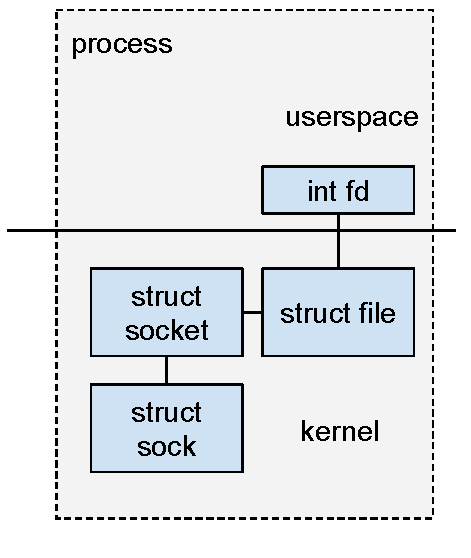
\includegraphics[width=\textwidth]{slides/networking-socket/socket_kernel.pdf}
		\column{0.7\textwidth}
		\begin{itemize}
			\item Sockets have a \textbf{file descriptor}
			\item It is handled internally with a \textbf{pseudo file}
			\item \kstruct{socket} is the generic representation
				\begin{itemize}
					\item stores the SOCK\_xxx types
					\item holds the \kstruct{proto_ops} pointer
					\item interfaces with the syscall API
				\end{itemize}
			\item \kstruct{sock} is what the network stack manipulates
				\begin{itemize}
					\item more internal representation
					\item for use mostly by the network stack
					\item maintains the queues, locks, and internal state
				\end{itemize}
		\end{itemize}
	\end{columns}
	% schematic +  explanation
\end{frame}

\begin{frame}[fragile]{\kstruct{proto_ops}}
	\begin{columns}
		\column{0.5\textwidth}
			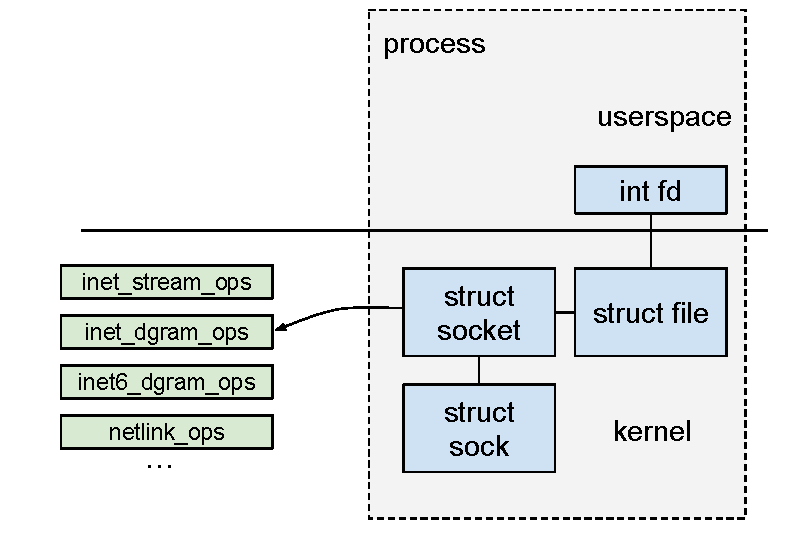
\includegraphics[width=\textwidth]{slides/networking-socket/socket_proto_ops.pdf}
		\column{0.5\textwidth}
		\begin{itemize}
			\item \kstruct{proto_ops} implement the protocol-specific operations
			\item Selected at socket creation based on the \textbf{family}
			\item Very close to the syscall interface
		\end{itemize}
		\begin{minted}{c}
struct proto_ops{
...
int (*bind) (struct socket *sock,
             struct sockaddr *myaddr,
             int sockaddr_len);
int (*sendmsg) (struct socket *sock,
                struct msghdr *m,
                size_t total_len);
...
};
		\end{minted}
	\end{columns}
\end{frame}

\begin{frame}{sending through a socket}
	\begin{enumerate}
		\item Userspace program calls \code{write()}, \code{send()}, \code{sendto()} or \code{sendmsg()} 
		\item The corresponding \code{syscall} is invoked
		\item All above syscalls end-up calling \kfunc{__sock_sendmsg}
		\item \code{sock->ops->sendmsg()} is called (\kfunc{inet6_sendmsg}, \kfunc{inet_sendmsg}, etc.)
		\item \code{sock->sk_prot->sendmsg()} is called (\kfunc{tcp_sendmsg}, \kfunc{udpv6_sendmsg}, etc.)
		\item \code{skb} chain gets created through \kfunc{ip_make_skb} or \kfunc{ip6_make_skb}
		\item \code{skb} is then sent with e.g.\kfunc{udp_send_skb}, which calls \kfunc{ip_send_skb}
		\item The target \kstruct{net_device} is retrieved with \kfunc{ip_route_output_key_hash}
			\begin{itemize}
				\item This is cached in \kstruct{sock}
			\end{itemize}
		\item \kfunc{dst_output} is eventually called, handing over from L4 to L3
	\end{enumerate}
\end{frame}

\begin{frame}{L3 processing}
	\begin{itemize}
		\item In \kfunc{ip_finish_output} or \kfunc{ip6_finish_output}
		\item The Layer 2 \textbf{MTU} is looked-up (\code{skb->dev->mtu})
		\item The \code{skb} is \textbf{fragmented} if needed
		\item Once the \textbf{routing} information is found, the \textbf{neighbour} is looked up
		\item This is usually done by looking up the gateway in the \textbf{ARP} table
			\begin{itemize}
				\item ARP tables can be dumped with \code{ip neigh} (or \code{arp})
			\end{itemize}
	\end{itemize}
\end{frame}



